\documentclass[slidescentered]{beamer}


%%%%%%%%%%%%%%%% PACKAGES %%%%%%%%%%%%%%%%
\usepackage{color}
\usepackage{polski}
\usepackage{multicol}
\usepackage{algorithmic}
\usepackage{amsmath}
\usepackage{mathabx}
\usepackage{xcolor}
\usepackage{dsfont}
\usepackage[utf8]{inputenc}

%%%%%%%%%%%%%%%% SETTINGS %%%%%%%%%%%%%%%%

\setbeamerfont{section in toc}{size=\normalsize}

\setbeamerfont{subsection in toc}{size=\tiny}


\AtBeginSection[]{
  \begin{frame}
  \vfill
  \centering
  \begin{beamercolorbox}[sep=8pt,center,shadow=true,rounded=true]{title}
    \usebeamerfont{title}\insertsectionhead\par%
  \end{beamercolorbox}
  \vfill
  \end{frame}
} 

%%%%%%%%%%%%%%%% THEME OPTIONS %%%%%%%%%%%%%%%%

\usetheme{Warsaw}
\usecolortheme{rose}

%%%%%%%%%%%%%%%% COMMANDS %%%%%%%%%%%%%%%%

\DeclareMathOperator*{\argmin}{arg\,min}
\newcommand\norm[1]{\left\lVert#1\right\rVert}
\newcounter{dummy}
\newcounter{dummy2}
\newtheorem{tw}{Twierdzenie}[dummy]
\newtheorem{uw}{Uwaga}
\newtheorem{fk}{Fakt}
\newtheorem{cel}{Cel}[dummy2]
\newtheorem{pr}{Problem}
\newcommand{\wek}[1]{
	{\bf #1} 
}

\newcommand{\todo}[1]{
	\LARGE{TODO: #1}
}

%%%%%%%%%%%%%%%% TITLE PAGE  EXEC %%%%%%%%%%%%%%%%

\title{Adaptacja macierzy kowariancji w metodach strategii ewolucyjnych}

\author[Eryk Warchulski]{\textbf{Eryk Warchulski} \newline \footnotesize{Opiekun pracy: \\ dr hab. inż. \textbf{Jarosław J. Arabas}, prof. PW}}
\institute[II]{\textit{Politechnika Warszawska \\
			Wydział Elektroniki i Technik Informacyjnych}}
\date{}

\begin{document}

%%%%%%%%%%%%%%%% TITLE PAGE  EXEC %%%%%%%%%%%%%%%%
\begin{frame}
	\titlepage
\end{frame}

%%%%%%%%%%%%%%%% TOC %%%%%%%%%%%%%%%%

\begin{frame}{Spis treści}
	\tableofcontents
\end{frame}


%%%%%%%%%%%%%%%% INTRO %%%%%%%%%%%%%%%%

\section{Metaheurystyki}
\subsection{Prefiks meta-}

\begin{frame}
	\begin{block}{Fakt}
		Heurystyka jest metodą przeszukiwania pewnej przestrzeni $\mathcal{S}$, która nie gwarantuje znalezienia rozwiązania optymalnego według przyjętego kryterium. 
	\end{block}
\pause
Przykłady przestrzeni $\mathcal{S}$:
\begin{itemize}
	\pause \item $\mathcal{S} = \mathbb{R}^{n}$
	\pause \item $\mathcal{S} = \mathbb{G}(V, E)$
	\pause \item $\mathcal{S} = \Sigma^{*}$
\end{itemize}
\end{frame}


\begin{frame}
	\begin{itemize}
		\item na początku XX wieku zaczęto stosować pojęcie \textit{metaheurystyki} bez podania ścisłej definicji 
		\pause
		\item w roku 2006 odbyła się pierwsza konferencja poświęcona metaheurystykom 
		\pause
		\item w dziedzinie tej panowała do pewnego momentu \textit{wojna paradygmatów}:
	\end{itemize}
	\begin{center}
		\textit{metaphor-centric} vs \textit{framework-centric} 
		\pause
	\end{center}
\end{frame}


\begin{frame}{Eksplozja publikacyjna}
	\begin{figure}[H]
	\centering
	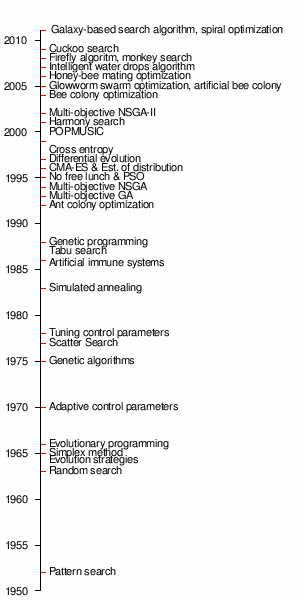
\includegraphics[width=0.5\textwidth, height=0.7\textheight]{./meta-algs.png}
	\caption{Oś czasu z datami publikacji nowych metod metaheurystycznych. Źródło [\ref{hist}].}
	\end{figure}
\end{frame}

\begin{frame}{Akcja-reakcja}

\begin{figure}[H]
	\centering
	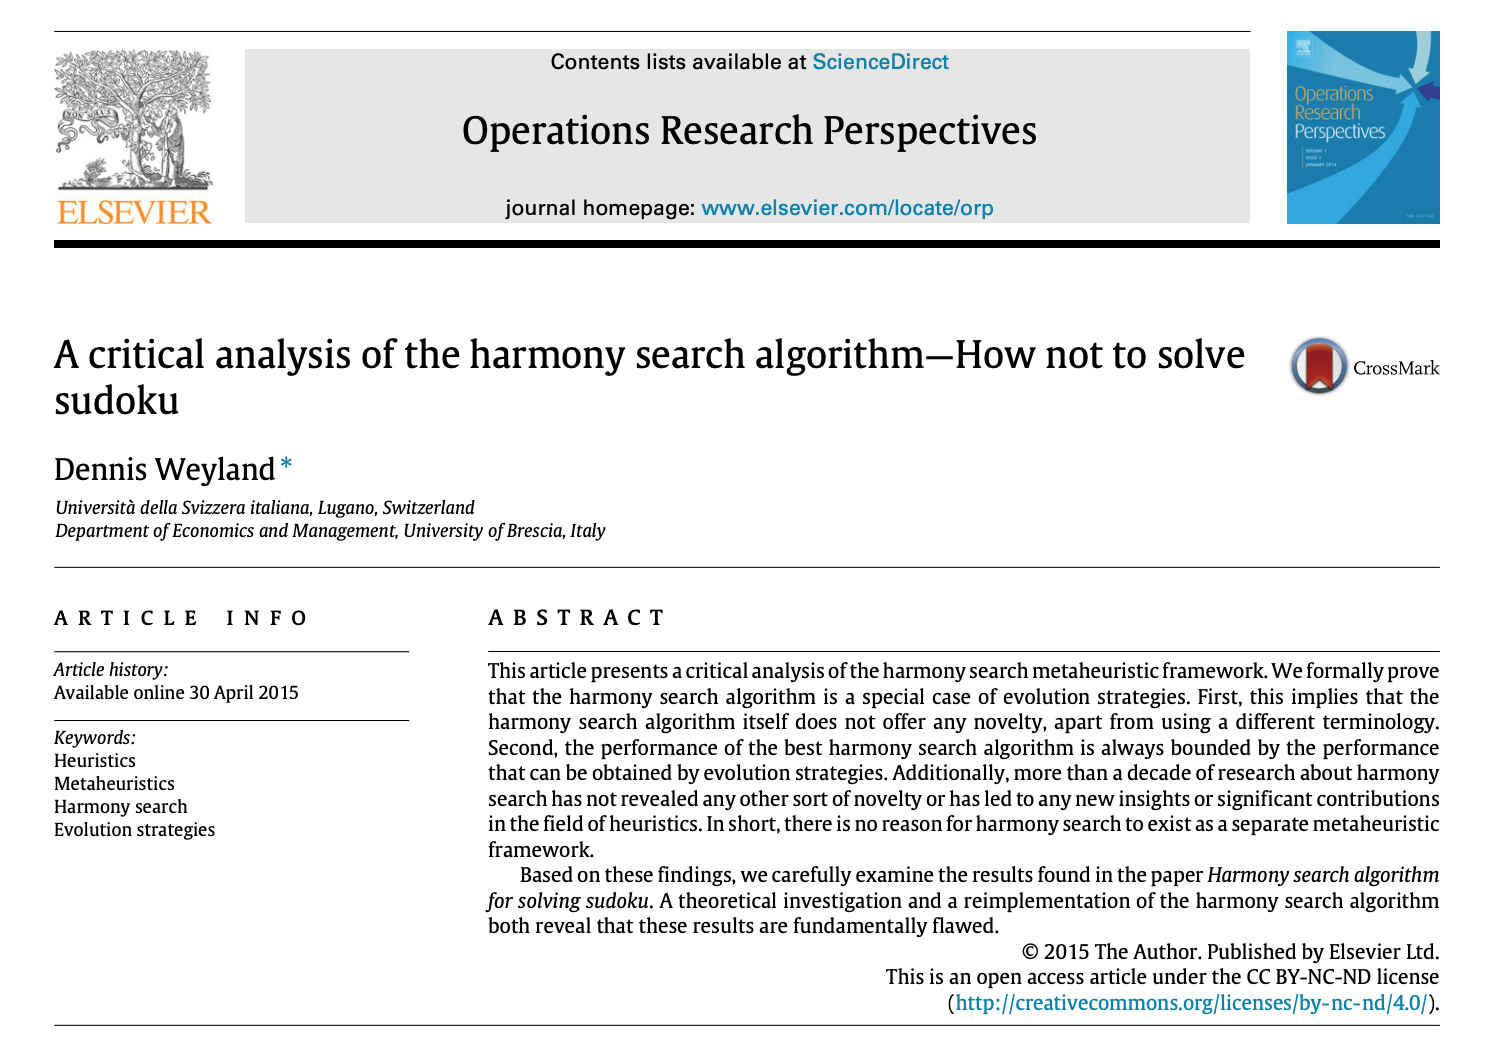
\includegraphics[width=0.85\textwidth, height=0.5\textheight]{./critic.png}
	\caption{Fragment krytycznego artykułu wobec metaheurystyk. Źródło [\ref{harmony}].}
\end{figure}

\end{frame}

\subsection{Istota pojęcia}
\begin{frame}{Podejście algebraiczne}
	\pause
	\begin{block}{Definicja}
		Metaheurystyka jest wysokopoziomowym podejściem do rozwiązywania problemów obliczeniowych. 
	\end{block}
	
	\pause Dla problemu $\mathcal{P}(D, Z)$, w którym $D$ nazywa się dziedziną problemu, a $Z$ przeciwdziedziną, przy pomocy zbioru operacji $\mathcal{O}$ poszukuje się rozwiązania tego problemu. \\
	\centering
	\pause Innymi słowy -- metaheurystyki to sposób myślenia o problemach w oderwaniu od ich reprezentacji.
\end{frame}

%%%%%%%%%%%%%%%% EVOl-COMP  %%%%%%%%%%%%%%%%

\section{Obliczenia ewolucyjne}
\subsection{Definicja}

\begin{frame}{Specyfikacja}
	\begin{multline}
		\text{typ}: EA(D, Z, M) \\
		\text{operacje}: \\
		\texttt{init}:  D x \mathbb{N} \rightarrow \text{Zbiór}(Z) \\
		\texttt{evol}: POP \rightarrow \text{Zbiór}(Z) \\
		\texttt{eval}: POP \rightarrow E \\
		\texttt{best}: POP \rightarrow Z \\
		\texttt{tune}: M \rightarrow M \\
		\texttt{aksjomaty}: z \in POP \implies  POP.eval(best()) \leq POP.eval(z) \\
	\end{multline}
\end{frame}

\begin{frame}

\begin{itemize}
	\pause \item	Operacja \texttt{init()} inicjalizuje zbiór rozwiązań dla problemu wejściowego $d \in D$, tj. \textbf{populację} \texttt{POP}, o pewnej liczebności $n \in \mathbb{N}$. 
	\pause \item	na zbiorze tym przeprowadzana jest operacja \textit{evol()} reprezentująca ewolucję, tj. iteracyjną procedurę stosowania operatorów ewolucyjnych jak \textbf{mutacja} lub \textbf{krzyżowanie}. 
	\pause \item na populacji przeprowadzona jest ewaluacja jej \textbf{osobników}, która przypisuje im \textbf{przystosowanie}. 
	\pause \item	algorytm ewolucyjny jest ponadto wzbogacony o zbiór parametrów $M$ charakteryzujących jego przebieg (np. wielkość populacji), który może ulegać zmianie w trakcie działania algorytmu.  
	\end{itemize}
\end{frame}


\subsection{Algorytmy genetyczne, programowanie genetyczne...}

\begin{frame}
\begin{itemize}
	\pause \item algorytm genetyczny Holland'a
	\pause \item programowanie genetyczne Kozy
	\pause \item ewolucja różnicowa Storn'a
	\pause \item programowanie ewolucyjne Fogel'a juniora 
	\pause \item neuroewolucja Fogel'a seniora
\end{itemize}
\end{frame}
\begin{frame}
	\begin{figure}[H]
		\centering
		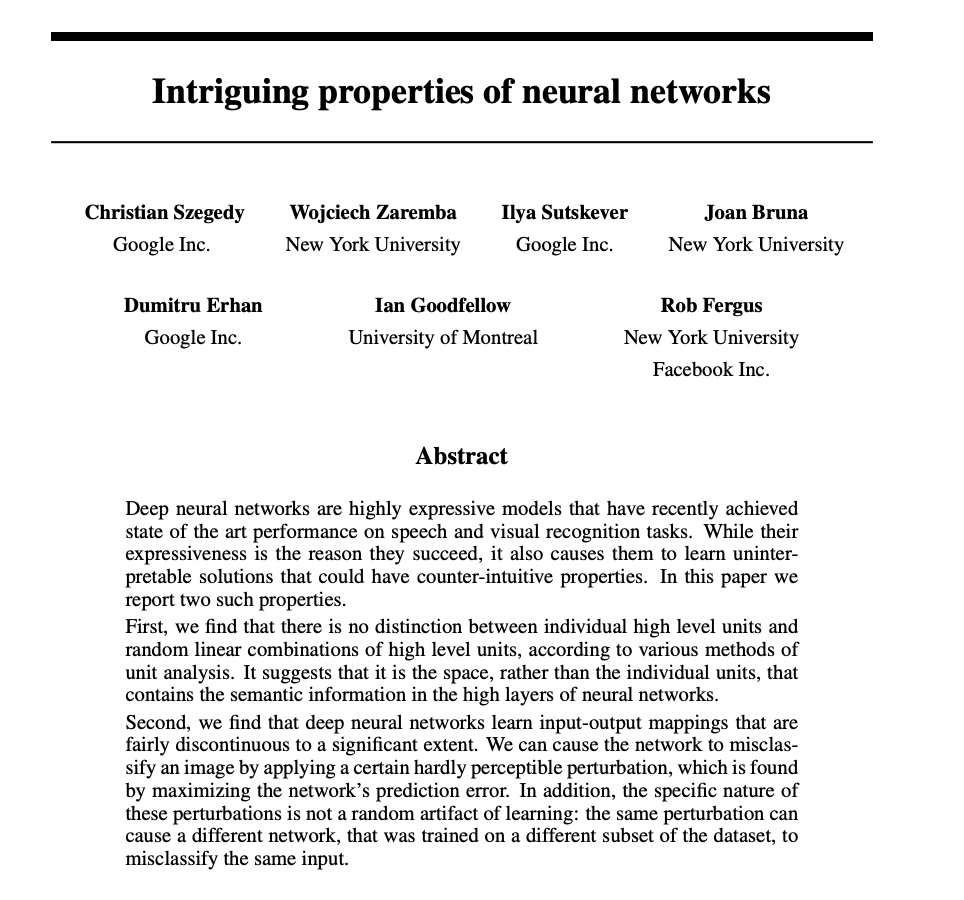
\includegraphics[width=0.5\textwidth, height=0.7\textheight]{./cnn.png}
		\caption{Fragment artykułu dotyczącego zaburzania konwolucyjnych sieci neuronowych. Źródło [\ref{cnn}].}
	\end{figure}
\end{frame}

\begin{frame}
\begin{figure}[H]
	\centering
	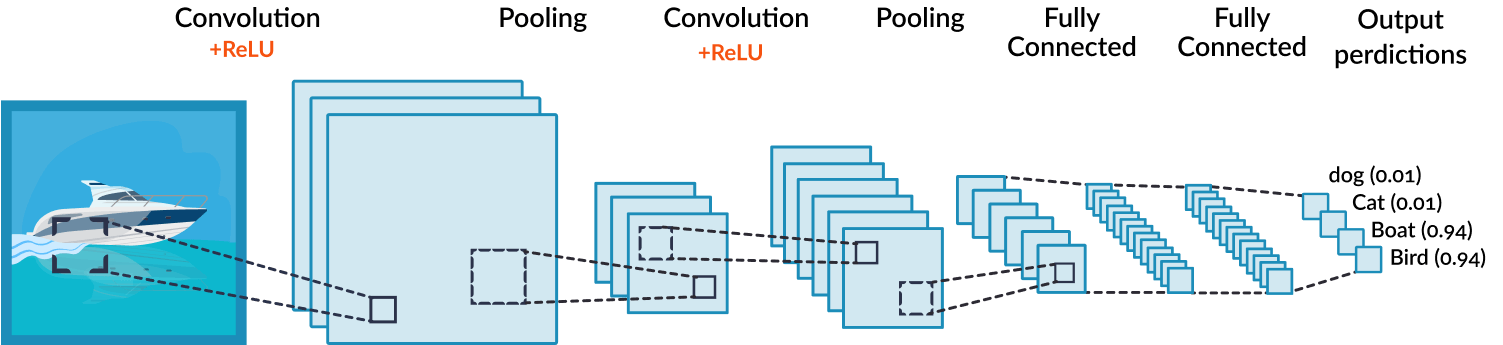
\includegraphics[width=0.9\textwidth, height=0.7\textheight]{./cnn-2.png}
	\caption{Architektura konwolucyjnej sieci neuronowej. Źródło: \texttt{Google Images}.}
\end{figure}
\end{frame}



%%%%%%%%%%%%%%%% EVOL STRAT  %%%%%%%%%%%%%%%%

\section{W stronę CMA}
\subsection{Strategie ewolucyjne -- początki}

\begin{frame}
	\begin{itemize}
	\item domena metody: $ D = \mathbb{R}^{\mathbb{R}^{p}}$ 
	\pause \item rezygnacja z krzyżowania $\texttt{evol} = \texttt{mut()}$
	\pause 	\item wyposażenie w samoadaptację $\texttt{tune}\colon POP x M \rightarrow M$ 
	\pause	\item bazowanie na rozkładzie normalnym $\mathcal{N}_p(\mu, \sigma^{2}\Sigma)$
	\end{itemize}
\end{frame}


\begin{frame}
	\begin{figure}[H]
		\centering
		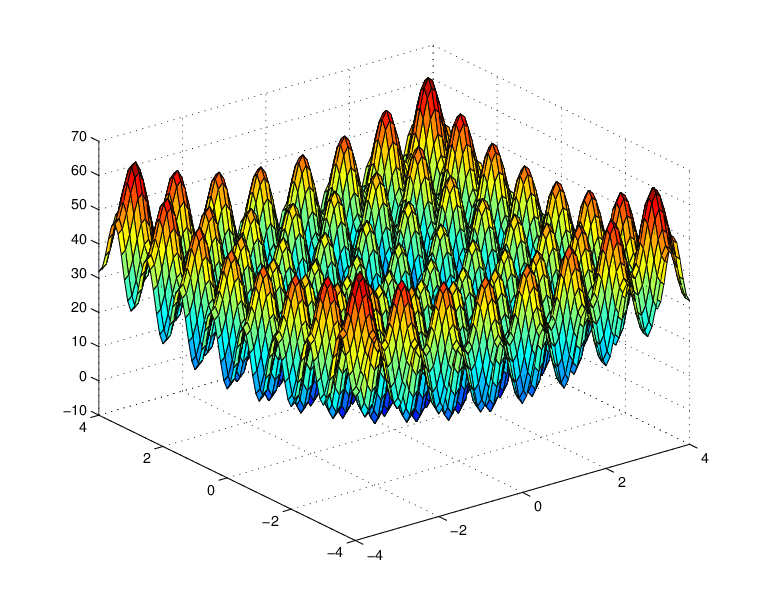
\includegraphics[width=0.7\textwidth, height=0.7\textheight]{./func-example.png}
		\caption{Przykład funkcji Rastrigina $f\colon \mathbb{R}^{2} \bigtimes \mathbb{R}$. Źródło: \texttt{Google Images}.}
	\end{figure}
\end{frame}

\subsection{Najlepsze losowanie}

\begin{frame}{Dlaczego rozkład normalny?}

	\begin{equation}
		x_{k} :=  m_{k} + \sigma_{k}\mathcal{N}_{p}(0, \Sigma), k \in \{1, \dots, \lambda\}
	\end{equation}
\end{frame}

\begin{frame}
	\begin{itemize}
	 	\item algorytm w początkowych iteracjach potrzebuje dużej różnorodości, aby móc sprawnie eksplorować przestrzeń przeszukiwań 
	\pause 	\item niewielka różnorodność zmniejsza prawdopodobieństwo znalezienia optimum globalnego
	\pause	\item ...rozkład normalny posiada największą entropię w klasie rozkładów ciągłych z nośnikiem $R^{p}$

	\pause 
	\end{itemize}
	\begin{equation}
		-\int_{X}\text{pdf}(x)\text{log}\{\text{pdf}(x)\}dx
	\end{equation}
\end{frame}

\begin{frame}
	\begin{figure}[H]
		\centering
		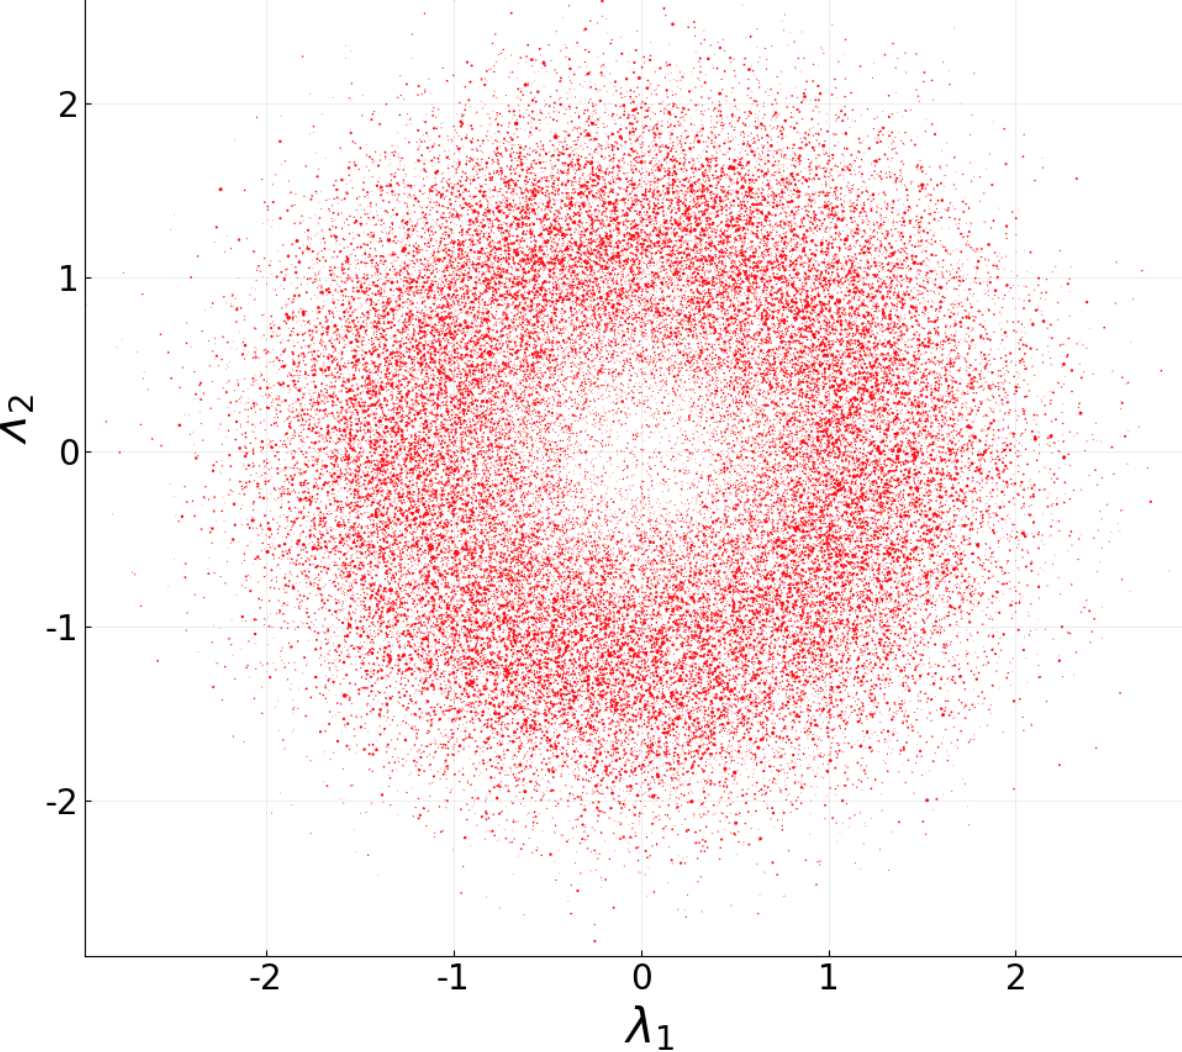
\includegraphics[width=0.7\textwidth, height=0.7\textheight]{./gauss-iso.png}
		\caption{Punkty wylosowane z izotropicznego rozkładu normalnego.\texttt{Google Images}.}
	\end{figure}
\end{frame}


\begin{frame}
	\begin{itemize}
		\item kształt rozkładu normalnego jest determinowany przez $\Sigma$
	\end{itemize}

	\pause Elipsoida koncentracji: 

	 \begin{equation}
		 \{x \in \mathbb{R}^{p}: (x-\mu)^{T}\Sigma^{-1}(x-\mu) = c \}
	 \end{equation}
\end{frame}
\begin{frame}
	\begin{figure}[H]
		\centering
		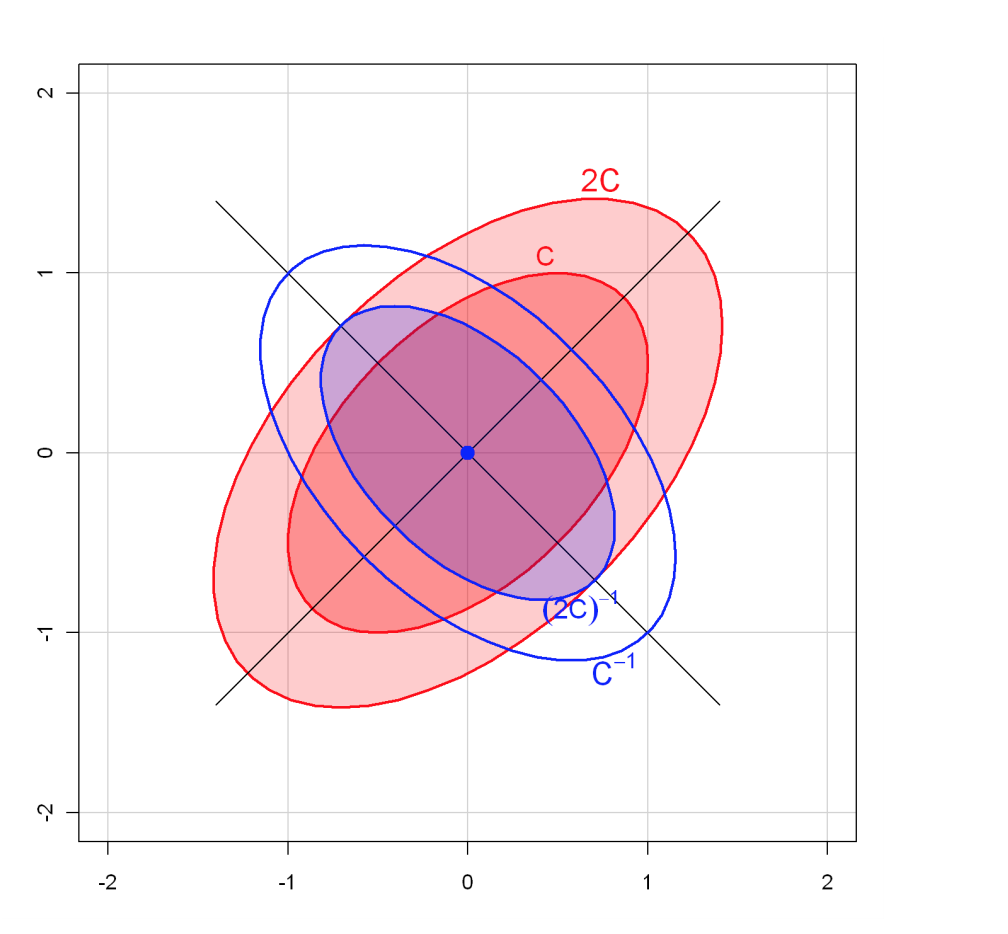
\includegraphics[width=0.7\textwidth, height=0.7\textheight]{./elipse-cov.png}
		\caption{Elipsoida kocentracji nie-izotropicznej macierzy kowariancji.\texttt{Google Images}.}
	\end{figure}
\end{frame}

\begin{frame}
	\begin{figure}[H]
		\centering
		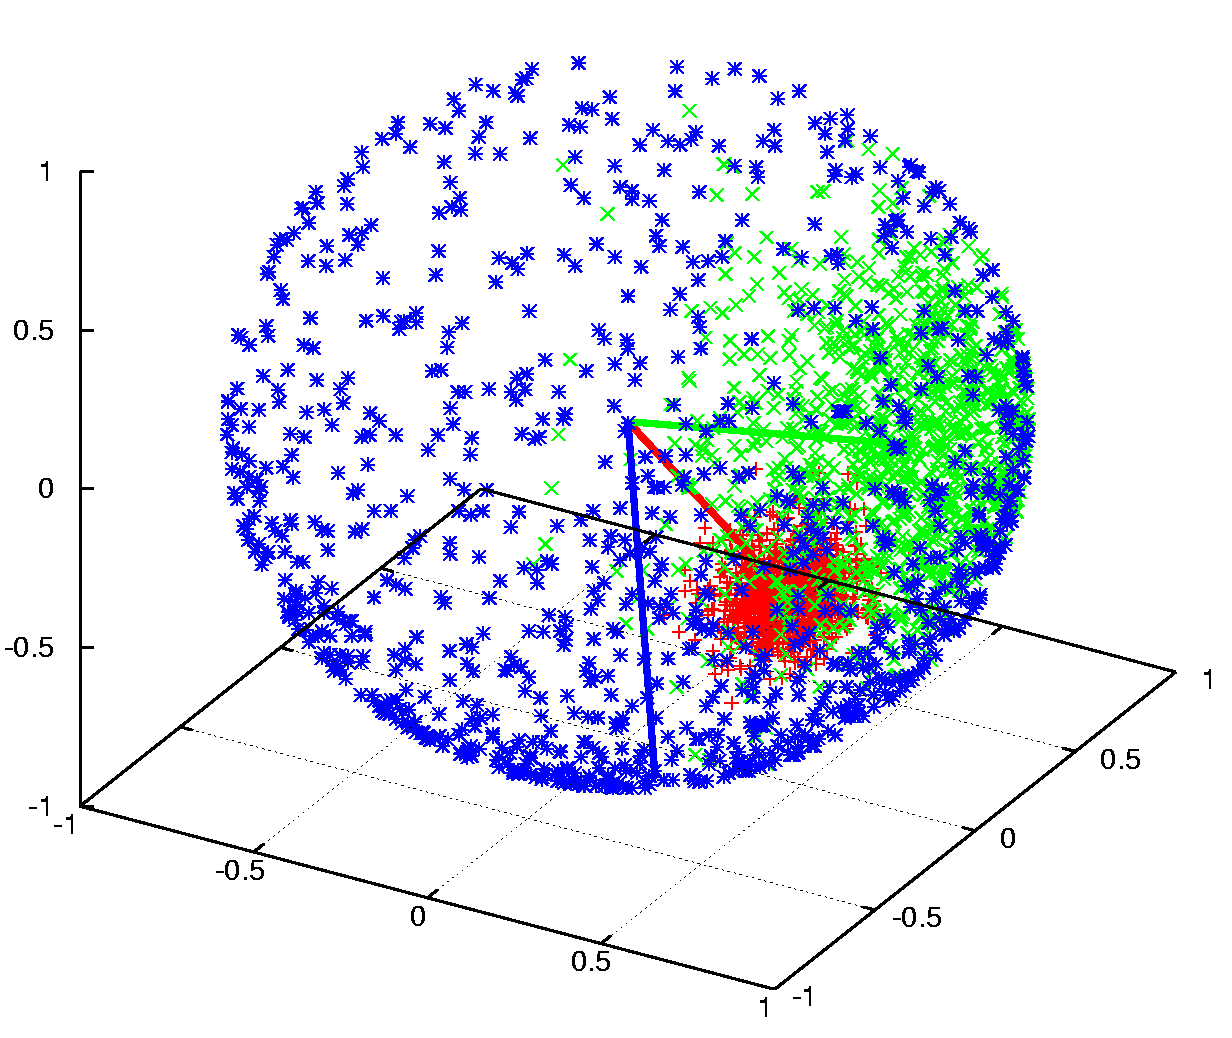
\includegraphics[width=0.7\textwidth, height=0.7\textheight]{./von-mises.png}
		\caption{Niesymetryczny rozkład kierunkowy Fishera-Misesa.\texttt{Google Images}.}
	\end{figure}
\end{frame}


\subsection{Samo-adaptacja}

\begin{frame}{Samoadaptacja metody}
	\begin{itemize}
		\item mechanizm metody, który ciężko wyprowadzić z podstaw statystycznych, które za nim stoją
	\pause 	\item wziąż oparty na heurystykach
	\end{itemize}
\end{frame}

\begin{frame}
	Prostsze heurystyki:
	\begin{itemize}
		\pause 	\item reguła $\frac{1}{5}$
		\pause \item meta-ewolucja
	\end{itemize}
	czy bardziej złożone jak \textbf{CSA} (ang. \textit{cumulative step-size adaptation}).
\end{frame}

\begin{frame}{CSA}
	\begin{block}{Definicja: \textbf{Ścieżka ewolucyjna}}
		Ścieżką ewolucyjną nazywa się $j$-wymiarowy wektor:
		\begin{equation}
			\wek{m}^{t} - \wek{m}^{t-j}
		\end{equation}
	\end{block}
\pause 
	\begin{block}{Definicja: \textbf{Ścieżka przeszukiwań}}
		Ścieżką przeszukiwań nazywa się wielkość: 
		\begin{equation}
			\wek{p}^{t+1}_{\sigma} = (C^{t})^{-\frac{1}{2}}\frac{\wek{m}_{t+1} - \wek{m}_{t}}{\sigma^{t}} + (1 - \gamma)\wek{p}^{t}_{\sigma}
		\end{equation}
	\end{block}
\end{frame}

\begin{frame}{CSA c.d}
Reguła aktualizacji:
	\begin{equation}
	\sigma^{t+1} = \sigma^{t}exp\LARGE\{\alpha\frac{\|\wek{p}^{t}_{\sigma}\|}{\mathcal{E}\|\mathcal{N}_{p}(0, \mathcal{I}_{p})\|} -1\LARGE\}
	\end{equation}

\end{frame}

\subsection{Adaptacja macierzy}

\begin{frame}{Estymacja macierzy kowariancji}
	\begin{equation}
		\Sigma^{t+1} = \frac{1}{\mu}\sum^{\mu}_{k = 1}(\wek{x}^{t}_{k} - \wek{m}^{t}_{k})(\wek{x}^{t}_{k} - \wek{m}^{t}_{k})^{T}
	\end{equation}
\end{frame}

\begin{frame}{Heurystyk ciąg dalszy}
	\begin{itemize}
	 	\item CMA-ES w wersji podstawowej wprowadza dwie dodatkowe reguły adaptacji macierzy kowariancji
			\begin{itemize}
	\pause 			\item użycie poprzedniej wartość macierzy: $\Sigma^{t}$
					\begin{equation}
						\Sigma^{t+1} = \frac{1}{\mu}\sum^{\mu}_{k = 1}(\wek{x}^{t}_{k} - \wek{m}^{t}_{k})(\wek{x}^{t}_{k} - \wek{m}^{t}_{k})^{T} + (1 - \alpha)\Sigma^{t}
					\end{equation}
		\pause 		\item użycie ścieżki ewolucyjnej w celu kompensacji straty informacji:
					\begin{equation}
						\wek{p}^{t}_{\Sigma}(\wek{p}^{t}_{\Sigma})^{T}
					\end{equation}
			\end{itemize}
	\end{itemize}
Finalnie:
	\pause \begin{equation}
		\Sigma^{t+1} = \frac{1}{\mu}\sum^{\mu}_{k = 1}(\wek{x}^{t}_{k} - \wek{m}^{t}_{k})(\wek{x}^{t}_{k} - \wek{m}^{t}_{k})^{T} + (1 - \alpha)\Sigma^{t} + \beta\wek{p}^{t}_{\Sigma}\wek{p}^{t}_{\Sigma}
	\end{equation}
\end{frame}

\section{Dalsze kroki i otwarte kwestie}

\begin{frame}
	\begin{itemize}
	 	\item wyznaczenie \textit{lepszych} estymatorów macierzy kowariancji i średniej
			\begin{equation}
				\Sigma = \delta S + (1-\delta)F
			\end{equation}
		\pause \item zbadanie wpływu rozkładów kierunkowych na zachowanie się algorytmu
	\end{itemize}
\end{frame}

\section{Bibliografia}
	\begin{enumerate}
		\item "Principled Design of Continuous Stochastic Search: From Theory to Practice", Anne Auger, Nikolaus Hansen 
		\item "An Algebraic Approach to Population-Based Evolutionary Algorithm Generation", Yujun Zheng
		\item "A History of Metaheuristics", Kenneth Sorensen et al.\label{hist}
		\item "Intriguing properties of neural networks", Ian Goodfellow et al. \label{cnn}
		\item "A critical analysis of the harmony search algorithm. How not to solve sudoku", Dennis Weyland \label{harmony}
	\end{enumerate}
\end{document}


